\chapter{Vijačenje z robotom Fanuc CR-7iA}%


\begin{mdframed}[backgroundcolor=green!20, shadow=true,roundcorner=8pt]
\vspace{-0.35cm}
	
\section{Cilj vaje}
	
Pri tej vaji boste spoznali:
\begin{itemize}
	\item aplikacijo vijačenja s sodelujočim robotom,
	\item programiranje robota Fanuc,
	\item kalibracijo orodja,
	\item določitev uporabniškega koordinatnega sistema,
	\item delo z digitalnimi izhodi.
\end{itemize}
	
\end{mdframed}

\section{Vijačenje z robotom}
Aplikacija avtomatiziranega vijačenja z robotom je v industriji precej razširjena aplikacija. Na robotu je nameščena vijačnik za vijačenje vijakov. Vijačnik je nadzorovan preko krmilne enota za vijačenje, običajno je potreben še podajalnik vijakov. Z uvajanjem sodelujočih robotov se zato pojavlja tudi potreba po sodelujoči aplikaciji avtomatiziranega vijačenja, kjer se pojavi tudi potreba po vijačnikih, ki so varni za uporabo v bližini človeka. Problematika avtomatiziranega vijačenja s sodelujočim robotom je, da imamo na varnem robotu nevarno orodje. Posledično to pomeni, da mora biti robot ograjen, saj aplikacija ni dovolj varna za sodelovanje s človekom. Glavni nevarnosti sta konica orodja ali vijaka in navor, ki je potreben za vijačenje.
V industriji je vedno več povpraševanja po avtomatiziranih opravilih, pri katerih bi lahko sodeloval tudi operater, vendar so ta zaradi nevarnih orodij težje izvedljiva. Zelo veliko zanimanje je tudi za varno vijačenje s sodelujočim robotom. Želja je, da bi si lahko robot in operater pri izvedbi naloge delila delovni prostor in po potrebi tudi sodelovala. Potreba je torej po dodatnem varnostnem sistemu, ki bi omogočal varno vijačenje in sodelovanje operaterja z robotom. Operaterju je potrebno fizično omejiti dostop do nevarnih delov, ki so prisotni pri vijačenju. Zaščita mora biti tudi senzorično podprta, da se v primeru kontakta z operaterjem lahko izvede ustavitev sistema.


\section{Struktura sistema}

Robotski sistem sestavlja sodelujoči robot Fanuc CR-7iA s krmilnikom Fanuc R-30iB Mate, set za robotsko vijačenje Kolver, varnostna zaščita za sodelujoče vijačenje.  Celotna konfiguracija je predstavljena na sliki \ref{fig:fanuc_sistem}.

\begin{figure}[!hbt]
	\centering
	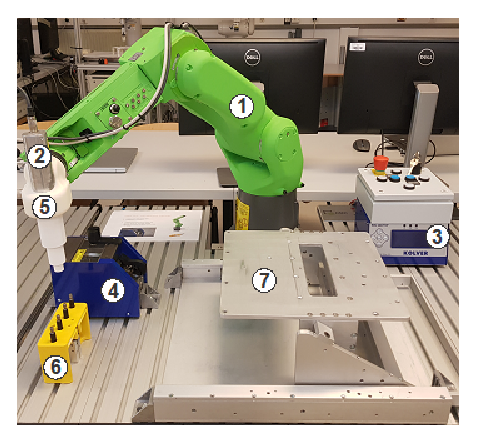
\includegraphics[width=0.75\textwidth]{sistem.eps}
	\caption{Prikaz uporabljenih naprav: 1 - robot Fanuc CR-7iA, 2 - vijačnik Kolver Pluto, 3 - krmilnik vijačnika Kolver, 4 - podajalnik vijakov Kolver, 5 - varnostni mehanizem, 6 - podajalnik orodja, 7 - obdelovanec.}
	\label{fig:fanuc_sistem}
\end{figure}

\subsection{Fanuc CR-7iA}

Fanuc CR-7iA robot je sodelujoči robot iz Fanucove družine sodelujočih robotov (slika \ref{fig:fanuc_druzina}). 

\begin{figure}[!hbt]
	\centering
	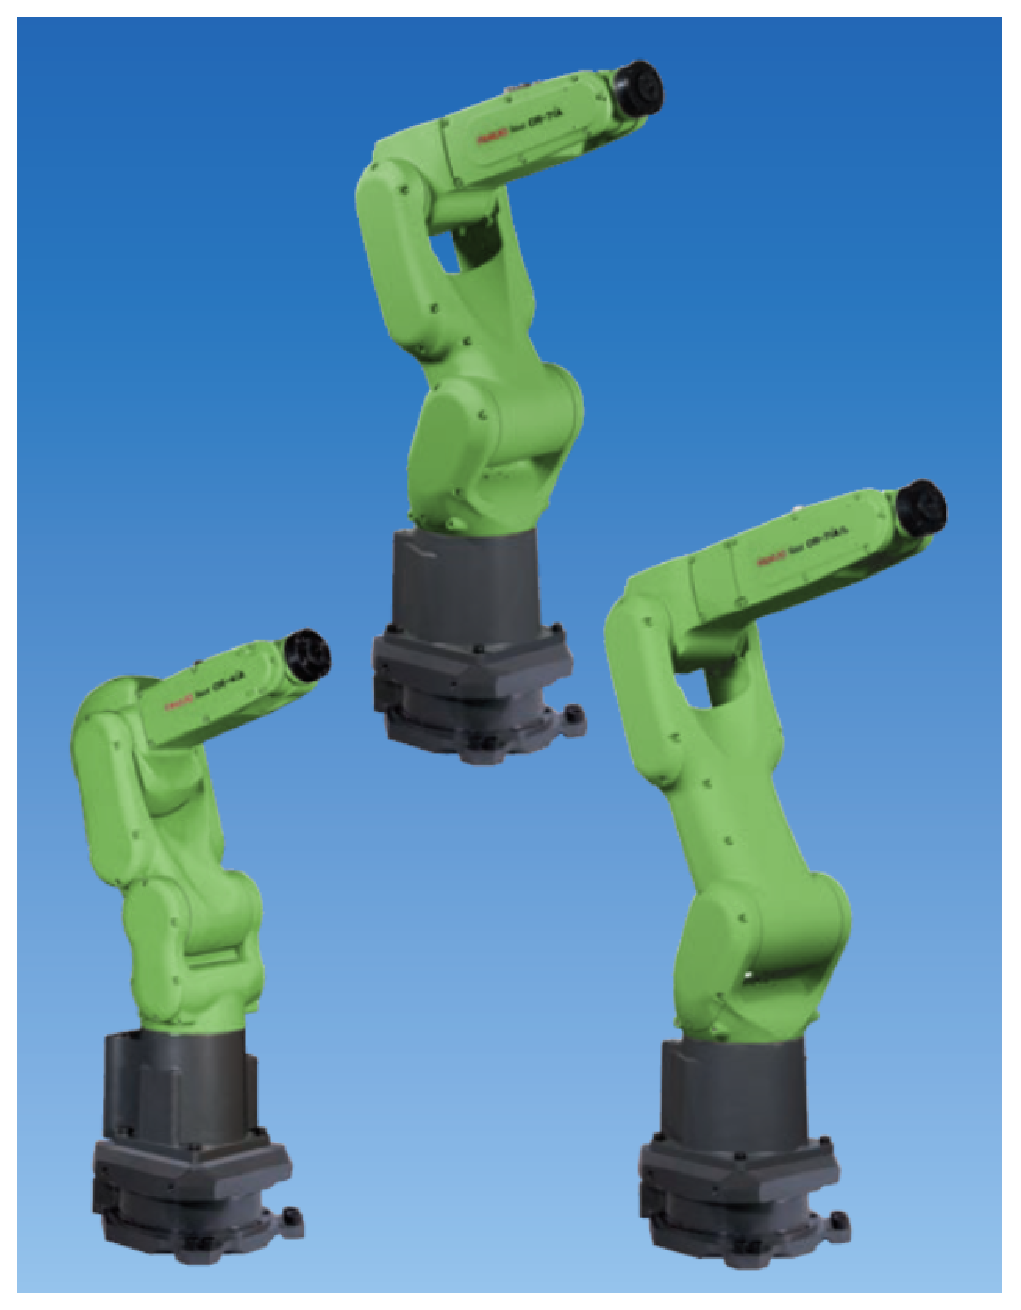
\includegraphics[width=0.4\textwidth]{CR_druzina.eps}
	\caption{Družina Fanuc sodelujočih robotov (CR-4iA, 7iA, 7iA/L)}
	\label{fig:fanuc_druzina}
\end{figure}

Robotska roka je antropomorfne oblike s 6 prostostnimi stopnjami. Robot ima doseg $717$ $mm$ in nosilnost $7$ $kg$. V osnovi gre za industrijskega robota Fanucove družine LR Mate, ki je opremljen z dodatnimi senzorji za merjenje sil, ki delujejo na robota, predvsem pa s prenovljenim krmilnikom, ki vsebuje vse potrebne varnostne sklope potrebne za sodelujočega robota. Robot je certificiran v skladu s standardom ISO 10218-1. To pomeni, da lahko človek in robot opravljata naloge v istem delovnem prostoru, oziroma lahko tudi sodelujeta med sabo. Robot se lahko zaradi ustrezne senzorije in vodenja ustavi, ko pride do dotika med človekom in robotom. 

Robot Fanuc je voden s krmilnikom Fanuc R-30iB Plus, ki se nahaja v omarici srednje velikosti. Krmilnik je opremljen z ročno učno enoto iPendant. 

Osnovni podatki robotske roke so podani v tabeli \ref{fig:specifikacije}, slika \ref{fig:delovni_prostor} prikazuje delovni prostor robota, slika \ref{fig:fanuc_osi} pa osi robota.

\begin{figure}[!hbt]
	\centering
	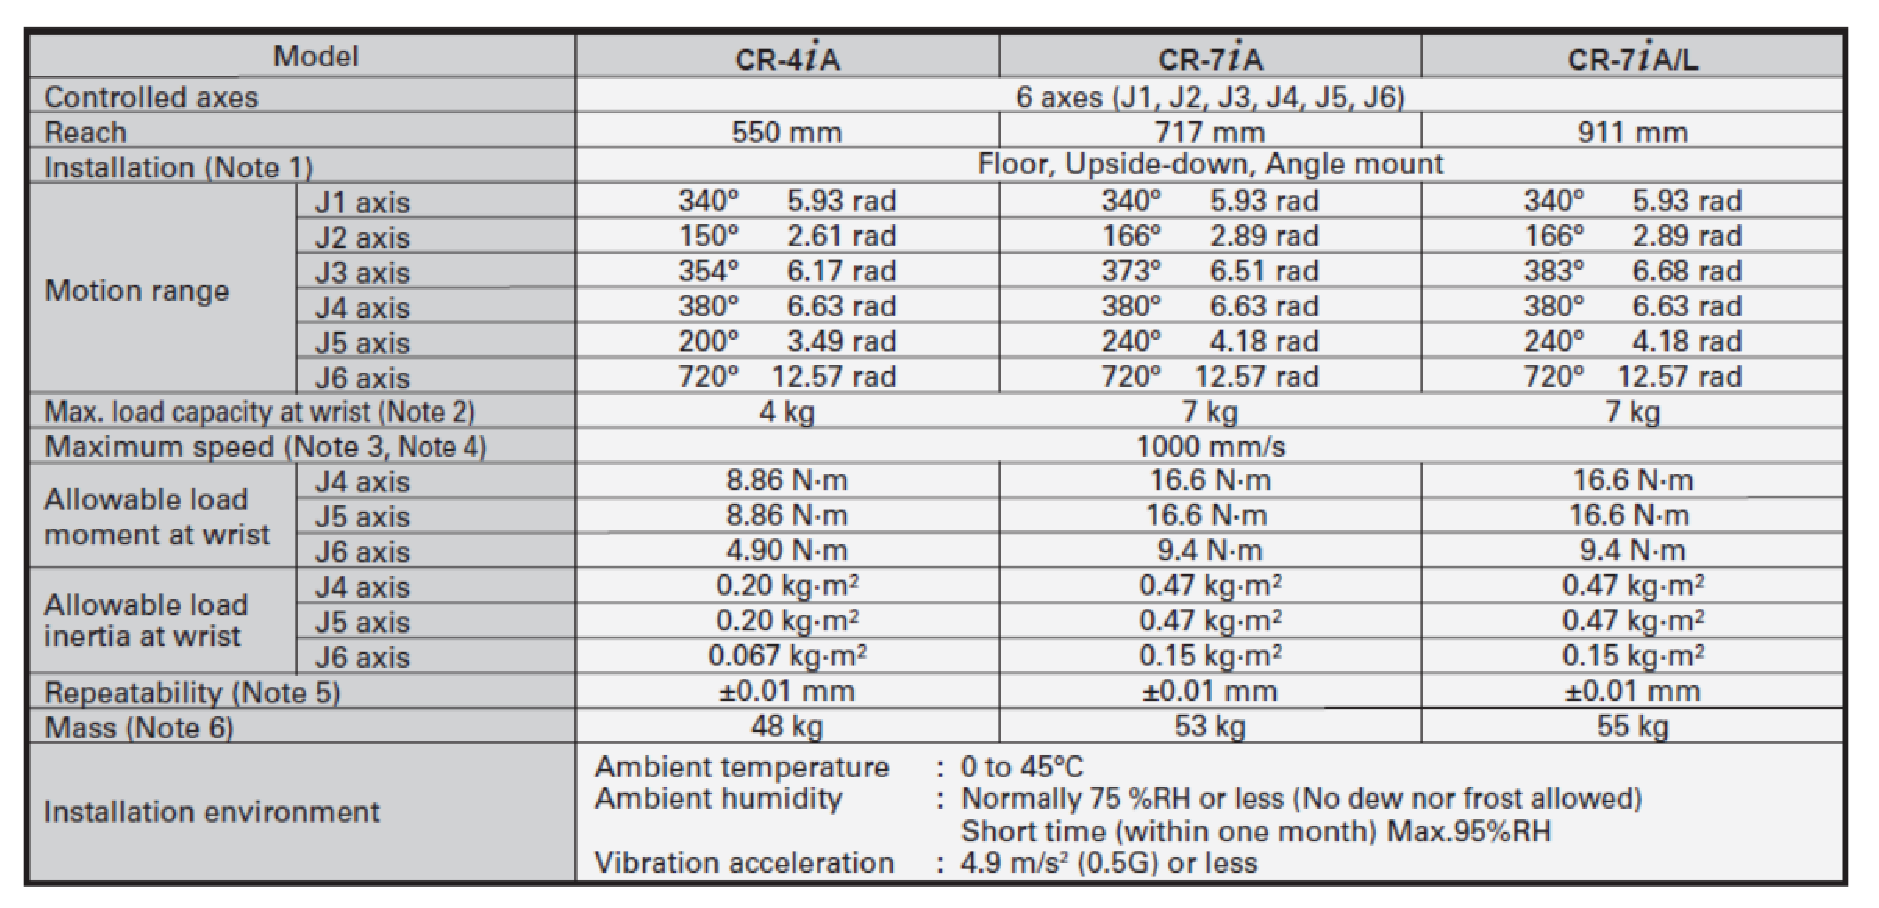
\includegraphics[width=1.0\textwidth]{specifikacije.eps}
	\caption{Specifikacije družine Fanuc sodelujočih robotov (CR-4iA, 7iA, 7iA/L)}
	\label{fig:specifikacije}
\end{figure}

\begin{figure}[!hbt]
	\centering
	\begin{minipage}{0.5\textwidth}
		\centering
		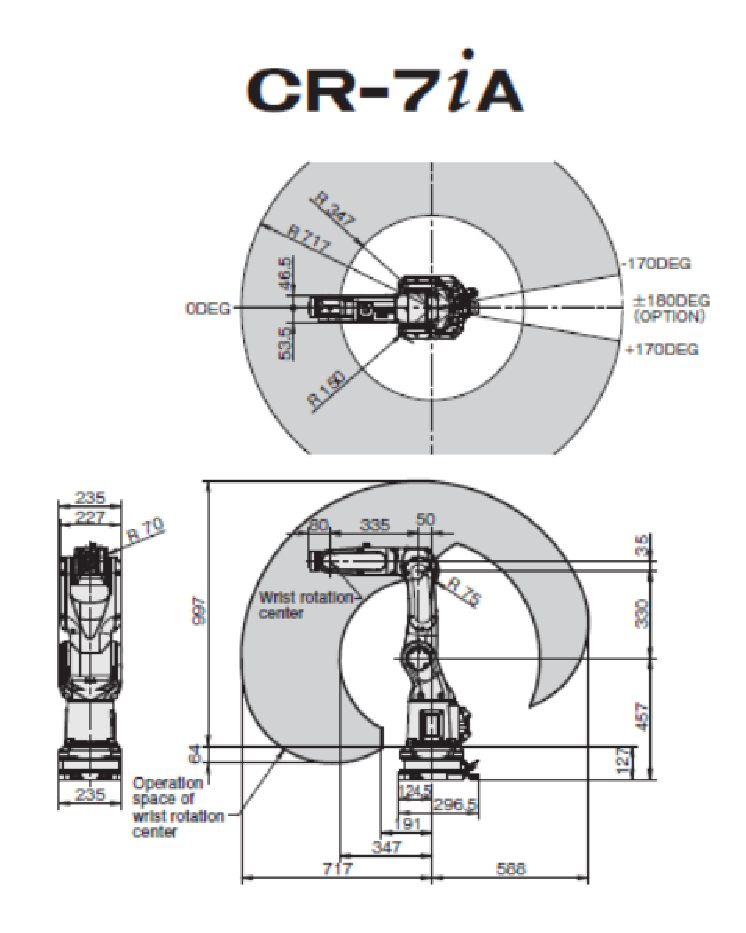
\includegraphics[width=1.0\textwidth]{delovni_prostor.eps}
		\caption{Delovni prostor robota 7iA.}
		\label{fig:delovni_prostor}
    \end{minipage}\hfill
	\begin{minipage}{0.5\textwidth}
		\centering
		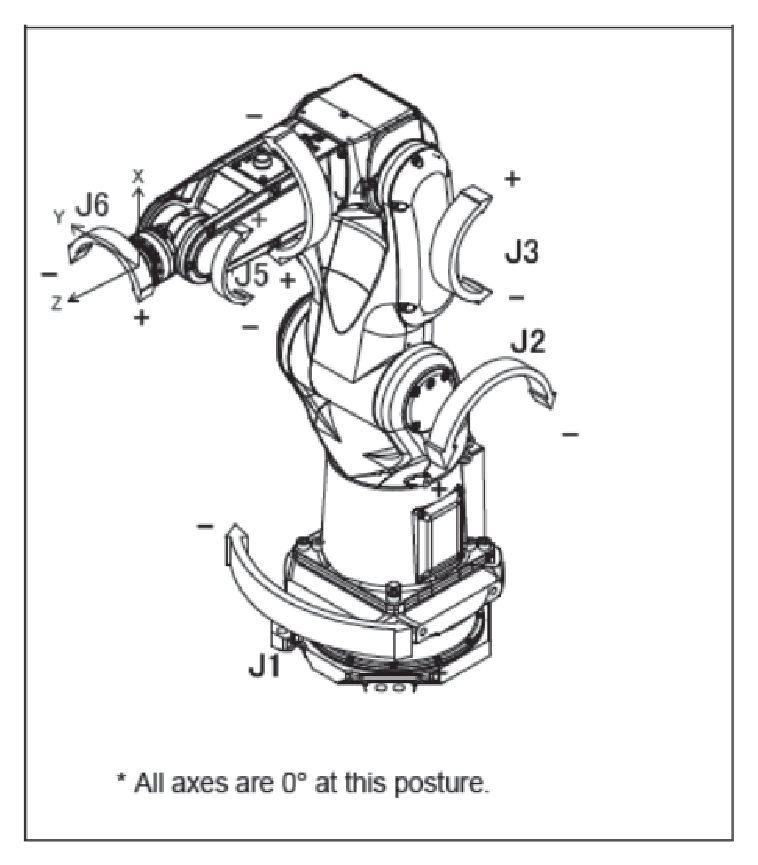
\includegraphics[width=1.0\textwidth]{fanuc_osi.eps}
		\caption{Osi robota 7iA.}
		\label{fig:fanuc_osi}
	\end{minipage}
\end{figure}

\newpage

\subsubsection{Varno delo z robotom}

Robot Fanuc CR-7iA je sodelujoči robot, kar pomeni, da se ob trkih z večjo silo samodejno ustavi, vendar je potrebno biti kljub vsemu previden pri delu z robotom. Robot Fanuc CR-7iA je razvit na podlagi klasičnega industrijskega robota, zato mehansko ni popolnoma prilagojen za inherentno varnost mehanske strukture. Še vedno so na robotu nevarna mesta, ki lahko povzročijo ukleščenje med segmente robota. Slika \ref{fig:uklescenje} prikazuje nevarna mesta za vkleščenje.

\begin{figure}[!hbt]
	\centering
	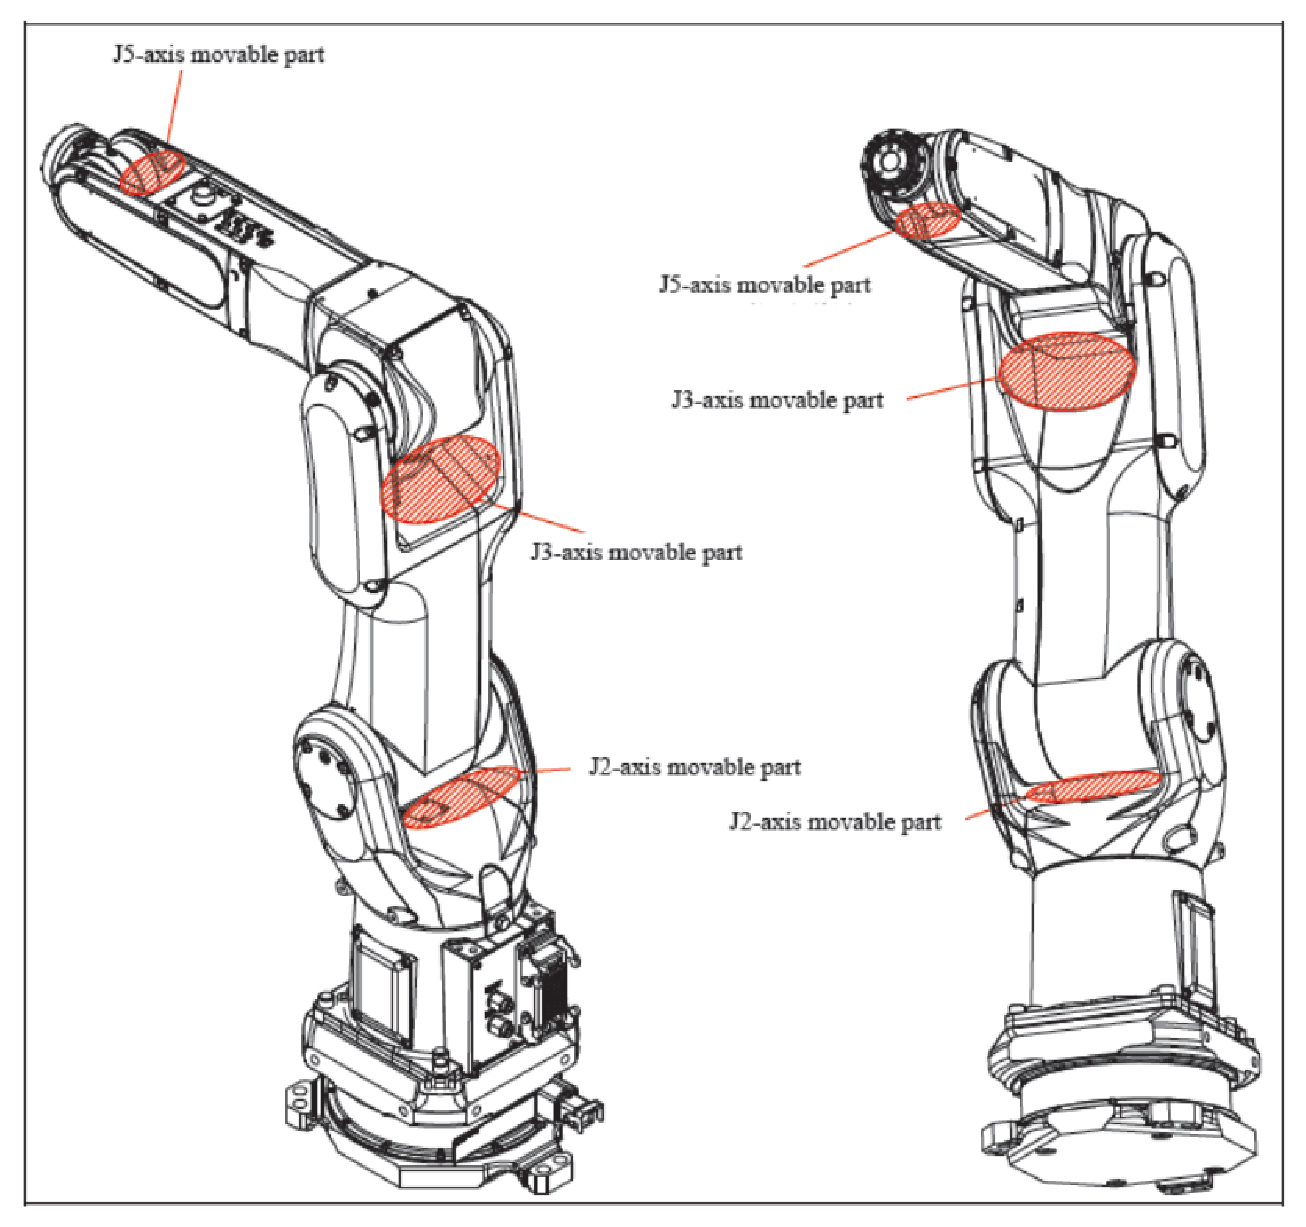
\includegraphics[width=0.4\textwidth]{uklescenje.eps}
	\caption{Možna mesta za ukleščenje med segmente robota.}
	\label{fig:uklescenje}
\end{figure}

Tako kot klasični roboti ima robot Fanuc tudi gumb za varnostno ustavitev na ohišju krmilnika in na ročni učni enoti (slika \ref{fig:em_stop}).

\begin{figure}[!hbt]
	\centering
	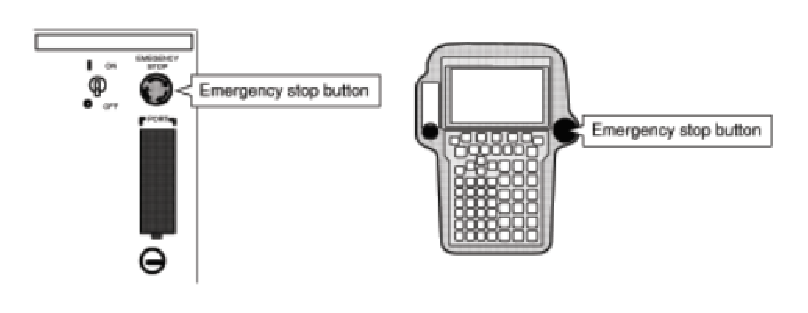
\includegraphics[width=0.5\textwidth]{em_stop.eps}
	\caption{Osi robota 7iA.}
	\label{fig:em_stop}
\end{figure}

\subsubsection{Ročna učna enota iPendant}

Učna enota se uporablja za programiranje robota. Ima barvni zaslon občutljiv na dotik, vendar priporočamo uporabo tipk na sami učni enoti. 
Slika \ref{fig:iPendant} prikazuje učno enoto na kateri so označene glavne skupine tipk:

\begin{itemize}
	\item Izklop v sili (rdeč okvir).
	\item Funkcijske tipke F1 do F5 (rumen okvir): najpogosteje se uporabljajo za izbiro gumbov na zaslonu, ki se pojavijo na dnu zaslona.
	\item Tipke za premikanje robota (oranžen okvir): s tipko COORD izberete tip koordinatnega sistema v katerem želite premikati robota, s tipkami potem robota premikate po posameznih oseh. Za premikanje robota morate najprej pritisniti varnostno tipko na spodnji strani učne enoto, izbrati tipko RESET. S tem prižgete motorje robota. Nato držite tipko SHIFT in s tipkami za premikanje robota premikate robota po izbrani osi.
	\item Tipka MENU: z njo prikličete na zaslon glavni meni.
	\item Tipka SHIFT.
	\item Tipka RESET.
	\item Tipka COORD: uporablja se za izbiro načina premikanje robota. Izbirate med načinom gibanja po:
	\begin{itemize}
		\item JOINT: gibanje po sklepih.
		\item WORLD: gibanje po oseh baznega koordinatnega sistema.
		\item TOOL: gibanje po oseh koordinatnega sistema izbranega orodja.
		\item USER: gibanje po oseh uporabniškega koordinatnega sistema, običajno ga definiramo tako, da je vezan na enega od objektov v delovnem prostoru robota.
		\item JGFRM: gibanje po oseh JOG FRAME koordinatnega sistema. JOG FRAME koordinaten sistem je poseben tip uporabniškega koordinatnega sistema, ki je definiran samo za gibanje, če se pojavi potreba, da moramo definirati koordinatni sistem, ki ga želimo uporabljati samo za gibanje. Privzeti koordinatni sistem je kar WORLD koordinatni sistem.
	\end{itemize}
	\item Tipki za spreminjanje hitrosti. Hitrosti je mogoče določati v procentih maksimalne hitrosti. Ko se pomaknete pod 1\% hitrosti, je naslednja nižja hitrost FINE, ki omogoča majhne inkrementalne pomike. Za FINE pomiki je še način VFINE, ki omogoča še manjše inkrementa pomika.
	\item Smerne tipke (zelen okvir) za pomik po menijih in izbiro možnosti.
	\item Tipki PREV in NEXT  za premikanje med nivoji oken.
	\item Tipke TEACH (SELECT, EDIT, DATA; moder okvir) so tipke za urejanje programa.
\end{itemize}

\begin{figure}[!hbt]
	\centering
	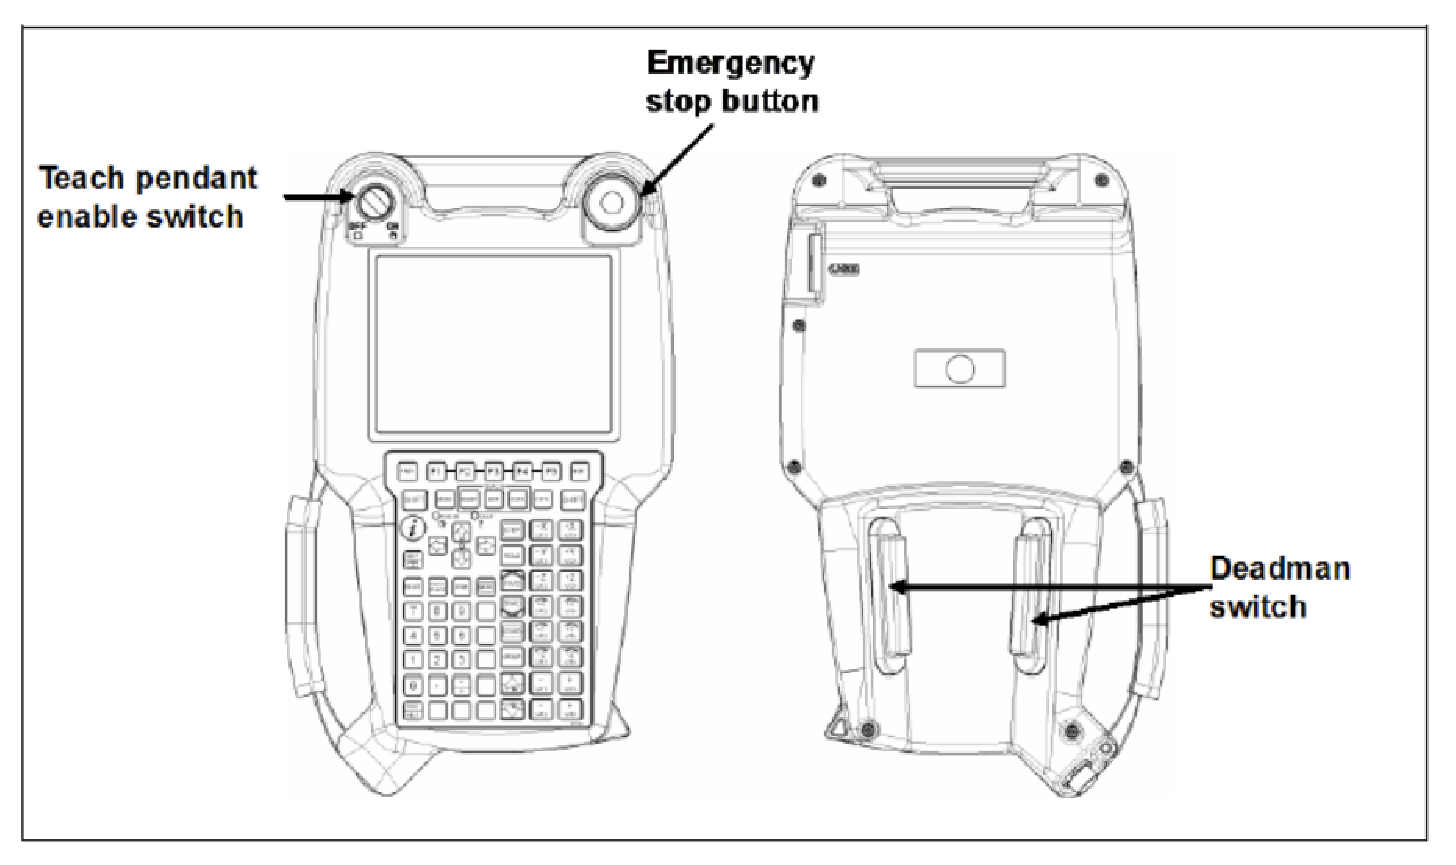
\includegraphics[width=0.75\textwidth]{pendant_ew_switch.eps}
	\caption{Prikaz glavnih varnostni stikal in tipk: tipka za izklop v sili, stikalo za izklop motorjev.}
	\label{fig:pendant_ew_switch}
\end{figure}

\begin{figure}[H]
	\centering
	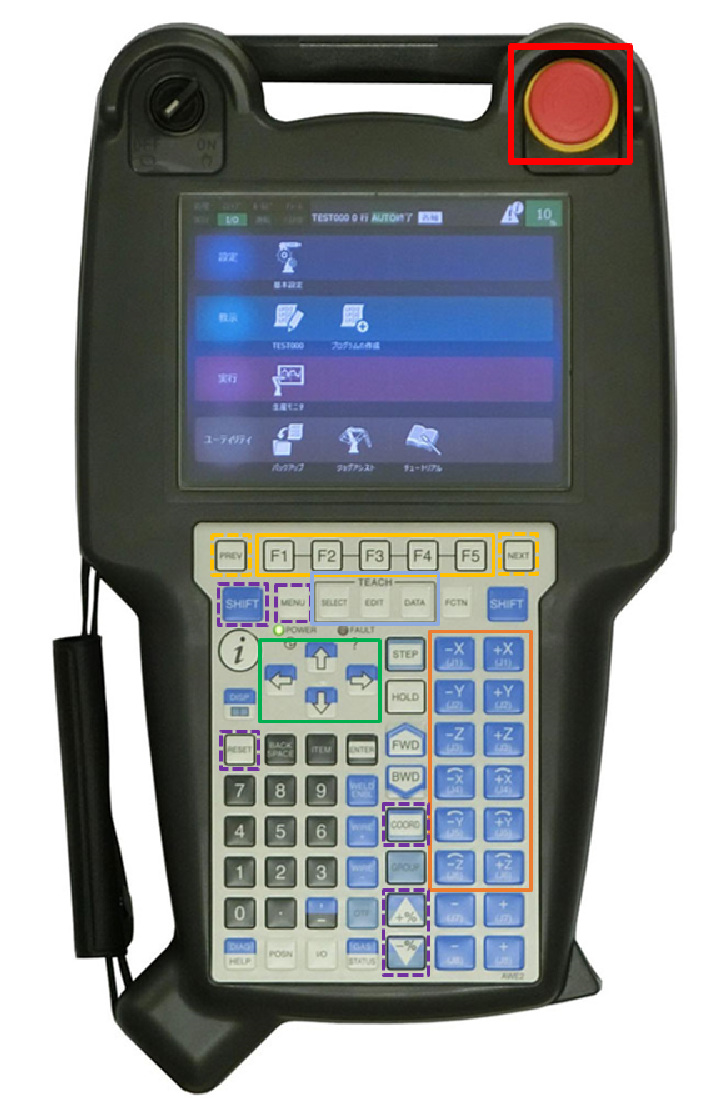
\includegraphics[width=0.95\textwidth]{iPendant.eps}
	\caption{Učna ročna enota iPendant.}
	\label{fig:iPendant}
\end{figure}

\newpage

\subsection{Sistem za vijačenje}

Sistem za vijačenje vključuje:
\begin{itemize}
	\item vijačnik KOLVER PLUTO 6CA (slika \ref{fig:kolver_vijacnik}),
	\item kontrolna enota za vijačnik je KOLVER EDU 2AE/TOP (slika \ref{fig:kolver_krmilnik}),
	\item varnostni mehanizem vijačnika,
	\item podajalnik vijakov KOLVER NFK UNI (slika \ref{fig:kolver_podajalnik}),
	\item podajalnik orodja (slika \ref{fig:podajalnik_orodja}).
\end{itemize}

CA družina KOLVER PLUTO vijačnikov je razvita za avtomatizirano vijačenje. Enosmerni motor omgoča navor med 0.85 do 6 Nm navora. Kontrolna enota za vijačnik je KOLVER EDU 2AE/TOP (https://kolver.it/products-list/8-Controllers-EDU-series) in je prikazana na sliki. Namen kontrolne enote je ustrezno napajanje vijačnika in nadzor nad ustreznim navorom za vijačenje. Na krmilniku se vnaprej določijo zahteve za vijačenje posameznega vijaka. Nato se proži program, ki ga potrebujemo. 

Za dodatno varnost smo v Laboratoriju za robotiko razvili varnostni mehanizem vijačnika in v sistem vključili nadzorni PLC krmilnik Siemens. Nadzorni sistem se uporablja za vodenje varnostnega mehanizma in za nadzor delovanja robota ter krmilnika vijačnika.

Zaradi vijačenja z različnimi nastavki smo v aplikacijo vključili tudi podajalnik orodja, ki smo ga načrtali v Laboratoriju za robotiko.

\begin{figure}[!hbt]
	\centering
	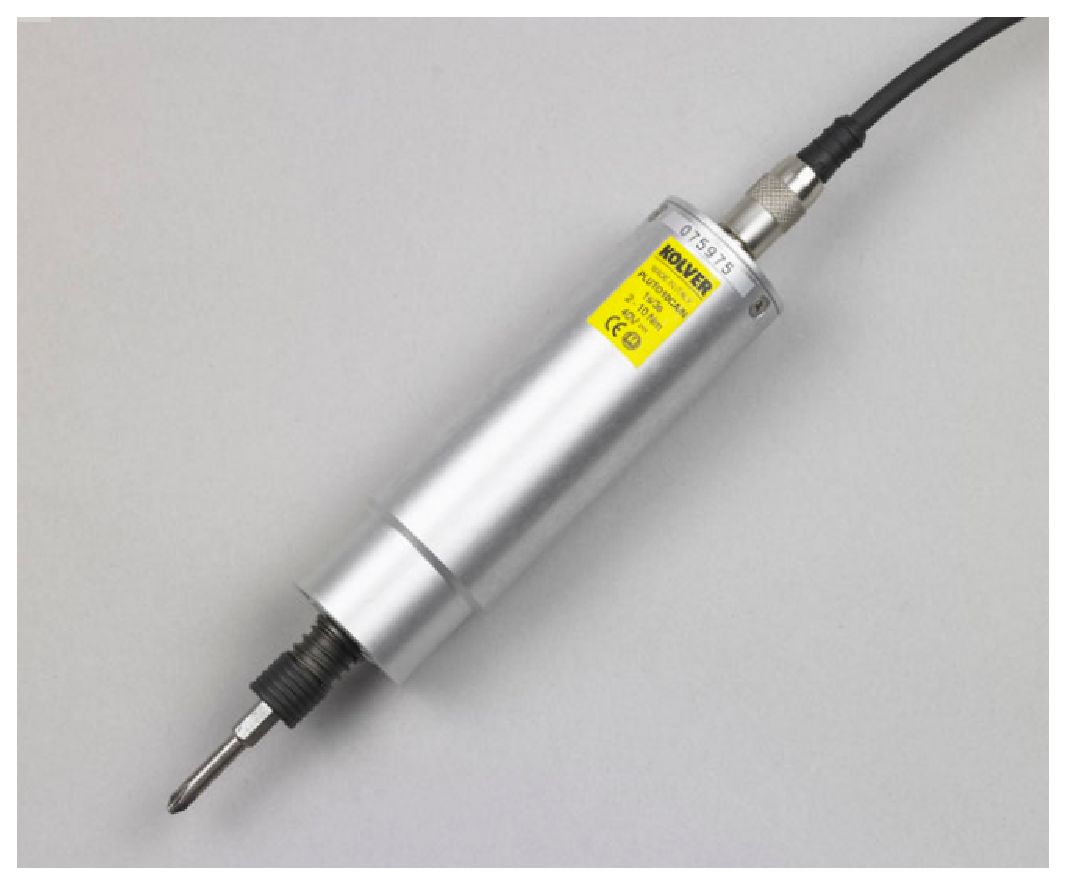
\includegraphics[width=0.5\textwidth]{kolver_vijacnik.eps}
	\caption{Vijačnik KOLVER PLUTO 6CA.}
	\label{fig:kolver_vijacnik}
\end{figure}

\begin{figure}[!hbt]
	\centering
	\begin{minipage}{0.45\textwidth}
		\centering
		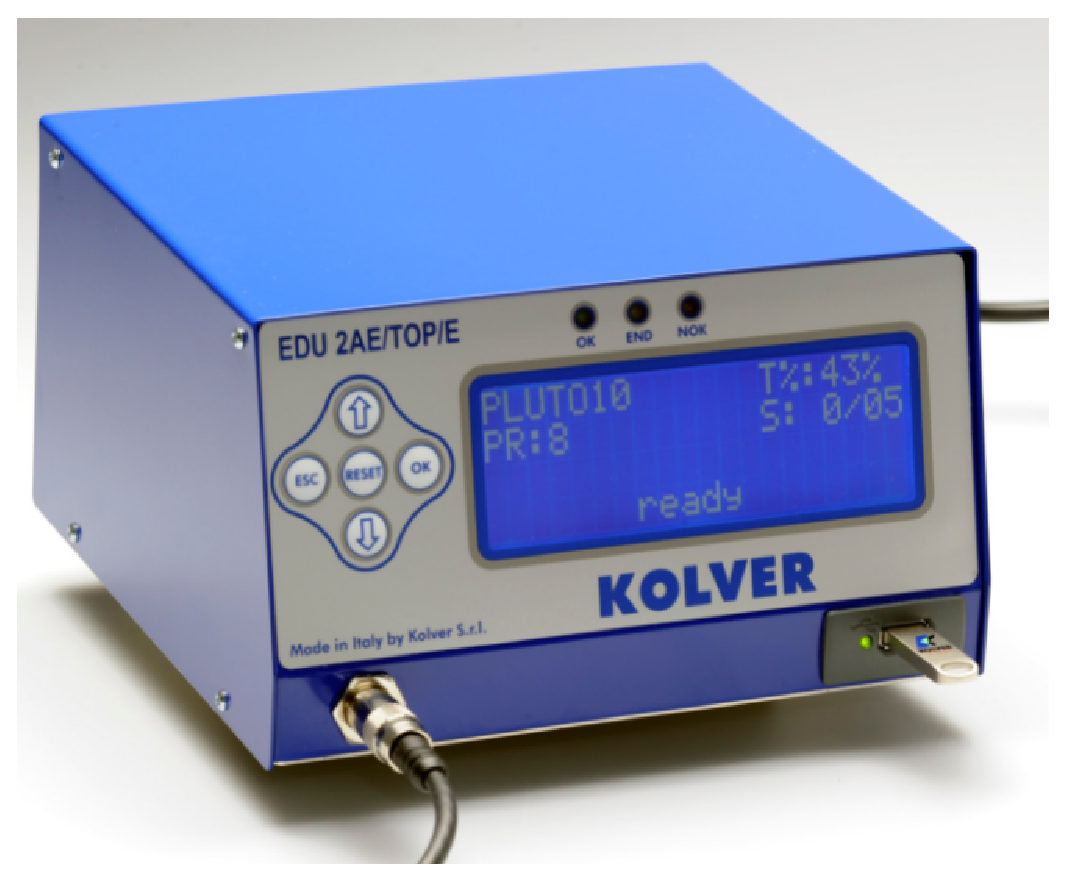
\includegraphics[width=1.0\textwidth]{kolver_krmilnik.eps}
		\caption{kontrolna enota za vijačnik je KOLVER EDU 2AE/TOP}
		\label{fig:kolver_krmilnik}
	\end{minipage}\hfill
	\begin{minipage}{0.45\textwidth}
		\centering
		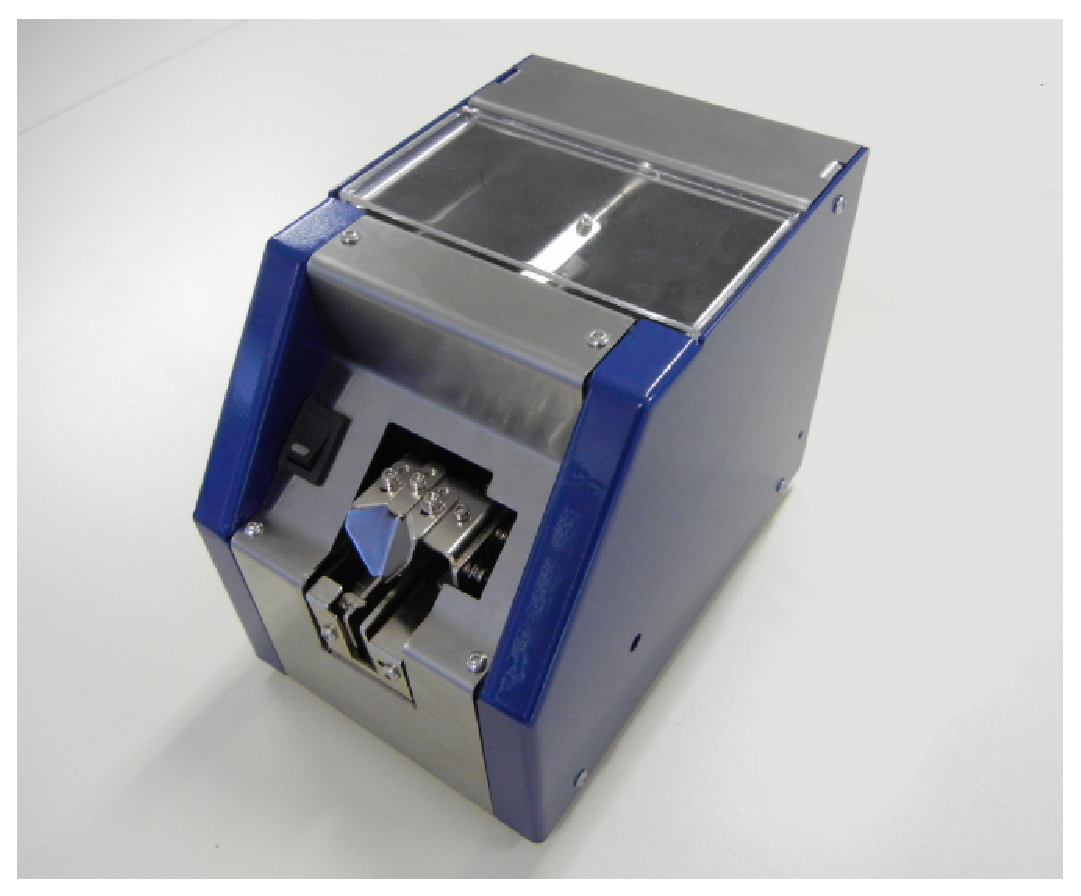
\includegraphics[width=1.0\textwidth]{kolver_podajalnik.eps}
		\caption{Osi robota 7iA.}
		\label{fig:kolver_podajalnik}
	\end{minipage}
\end{figure}

Podajalnik vijakov omogoča avtomatizirano podajanje vijakov vijačniku. Robot se mora z nameščenim vijačnikom pravilno približati podajalniku vijakov, nato se vijačnik vključi in pobere vijak, ki ga nato lahko privijači na želeno mesto. 

Zaradi vijačenja z različnimi nastavki je v aplikacijo vključen tudi podajalnik orodja oziroma nastavka (slika \ref{fig:podajalnik_orodja}). Nastavki za vijačenje so obdani s primerno oblikovanimi tulci z utori za lažji prijem. Za prijem nastavka skrbi pnevmatsko prijemalo, ki je skupaj s prsti vgrajeno v podajalno mizo. Prsti so primerno oblikovani, da zagotovijo zanesljiv prijem tulcev. Menjava nastavka poteka tako, da se z vijačnikom pri nizkih vrtljajih približujemo k nastavku. Ko se po obliki nastavek ujame z magnetnim podaljškom na vijačniku, prijemalo popusti in orodje se fiksira v podaljšek. Robot se nato z vijačnikom umakne in varnostni mehanizem pokrije nastavek za vijačenje. 

\begin{figure}[!hbt]
	\centering
	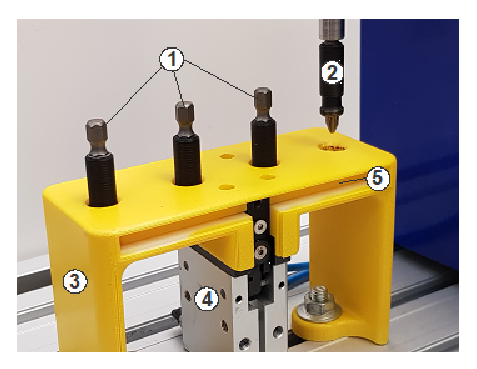
\includegraphics[width=0.55\textwidth]{podajalnik_orodja.eps}
	\caption{Podajalnika orodja: 1 - orodje za vijačenje, 2 - tulec, 3 - stojalo za orodje, 4 - pnevmatsko prijemalo, 5 - prsti prijemala za zaklep tulcev.}
	\label{fig:podajalnik_orodja}
\end{figure}

\newpage

\subsection{Integracija sistema}

Shema delovanja sistema je prikazana na sliki \ref{fig:shema_sistema}. Siemens krmilnik je centralna enota, ki skrbi za pravilno in varno delovanje celotnega sistema. Deluje kot nadzorni sistem. Krmilnik Fanuc je povezan s PLC krmilnikom povezan preko komunikacije Ethernet IP in preko digitalne varnostne vhodno-izhodne linije.  Robot je povezan tudi na podajalnik orodja, in sicer preko digitalnega izhoda. Varnostni mehanizem je povezan s krmilnikom PLC preko digitalne vhodno izhodne linije. Logika delovanja varnostnega mehanizma je na krmilniku PLC. To vključuje barvno osvetlitev in nadzor nad stanjem kontaktov v varnostnem mehanizmu.  Krmilnik vijačnika je prav tako povezan na nadzorni sistem preko digitalnih vhodno/izhodnih linij. Takšna vezava je smiselna zaradi varnosti pri vijačenju, saj je v nekaterih primerih ob ustavitvi robota treba zagotoviti, da se ustavi tudi vijačnik. Ob ponovnem zagonu pa je zaželeno, da se tudi vijačnik zažene nemoteno. S tem dosežemo, da je vijačenje zanesljivo, tudi če pridemo v kontakt z robotom med samim vijačenjem.

\begin{figure}[!hbt]
	\centering
	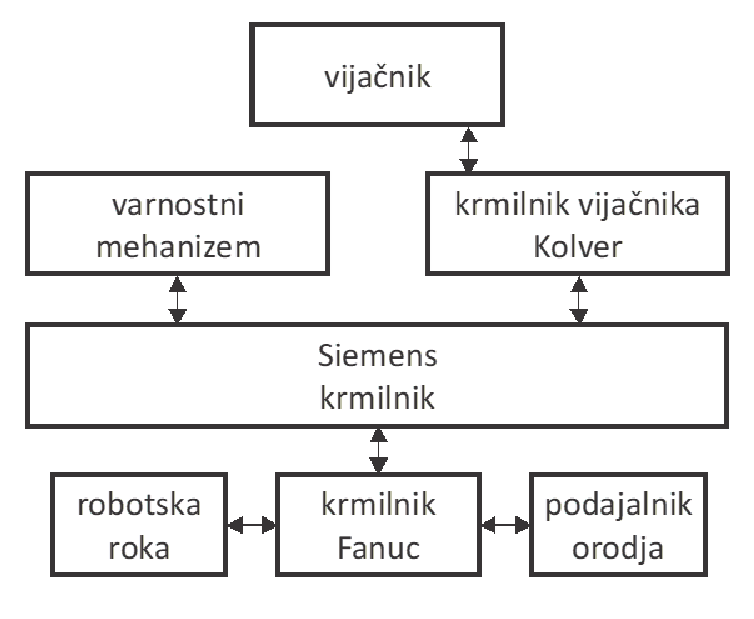
\includegraphics[width=0.65\textwidth]{shema_sistema.eps}
	\caption{Prikaz vezave celotnega sistema.}
	\label{fig:shema_sistema}
\end{figure}

\subsubsection{Tehnika pobiranja vijakov}

Glavna težava pri pobiranju vijakov je predvsem nezanesljiva lega in orientacija vijaka. Težava pa se pojavi tudi pri pobiranju vijakov z varnostnim mehanizmom, ki prekriva orodje. Težavo z varnostnim mehanizmom je rešena tako, da ga z distančnikom, ki je razviden iz slike \ref{fig:fanuc_sistem}, odmaknemo. Distančnik je primerno oblikovan, da omogoča pobiranje vijaka pod različnimi nakloni vijačnika. 

Vijake se pobira z magnetnimi nastavki pod naklonom $80^{\circ}$. Pristop pobiranja je takšen, da robot v neposredni bližini glave vijaka pri velikih hitrostih vrtenja vijačnika počasi spušča orodje. Orientacija in lega vijaka se tako prilagodil legi orodja. Izkaže se namreč, da je takšen pristop manj občutljiv na lego vijaka.   

\subsubsection{Tehnika vijačenja vijakov}
Ko robot pobere vijak, se z vijačnikom postavi nad navojno izvrtino, v katero bo vijačil. Ko je vijačnik dovolj blizu, da operater ne more poseči med varnostni mehanizem in površino ($D = 5$ $mm$), v katero vijačimo, se varnostni sistem vijačnika izklopi. V tem trenutku varnostni sistem sveti rdeče. Zažene se vijačnik in se s primerno hitrostjo linearno približuje izvrtini. Tik preden je vijak v celoti privijačen, izklopimo sodelujoči način robota, da lahko na vijak delujemo z večjo silo. 

Takoj, ko se vijačenje uspešno izvede, se sodelujoč način ponovno vključi. Vijačnik se umakne od točke vijačenja, nato pa se vključi tudi varnostni sistem vijačnika. Poudariti je treba, da je kljub izklopu sodelujočega načina programsko urejeno, da se robot ustavi, ko prekorači vnaprej določeno silo. V našem primeru je ta sila $60$ $N$. S tem preprečujemo, da bi lahko prišlo do mehanskih okvar v primeru, da se vijačenje ne bi uspešno izvedlo. 

\newpage

\section{Programiranje robota}

\subsection{Ročno vodenje robota}

Robota ročno vodimo s pomočjo ročne učne enote. 

\begin{mdframed}[backgroundcolor=yellow!20, shadow=true,roundcorner=8pt]

Za premikanje robota morate najprej pritisniti varnostno tipko na spodnji strani učne enoto (slika \ref{fig:enabl_device}), izbrati tipko RESET. S tem prižgete motorje robota. Nato držite tipko SHIFT in s tipkami za premikanje robota premikate robota po izbrani osi.

\end{mdframed}

\begin{mdframed}[backgroundcolor=yellow!20, shadow=true,roundcorner=8pt]
	
Trenutno lego robota preverite meniju Position. Do menija pridete preko tipke MENU, nato izberete \verb|0 NEXT|, sledi izbira menijske vrstice \verb|5 4D GRAPHICS|, ter nato \verb|2 Position Display| (glej sliko \ref{fig:menu_pos} (a)). Odpre se meni Position. V ukazni vrstici na dnu zaslona ((glej sliko \ref{fig:menu_pos} (b))) lahko izbirate med prikazi JNT (prikaz vrednosti v sklepih robota), USER (lega glede na izbrani uporabniški koordinatni sistem), WORLD (lega glede na koordinatni sistem robota).
	
\end{mdframed}

\begin{figure}[!hbt]
	\centering
	\psfrag{a}[r][r][1.0][0]{(a)}
	\psfrag{b}[r][r][1.0][0]{(b)}
	\includegraphics[width=1.0\textwidth]{meni_pos.eps}
	\caption{Dostop do prikaza lege robota.}
	\label{fig:menu_pos}
\end{figure}

Za vodenje imamo na voljo več koordinatnih sistemov:

\begin{itemize}
	\item JOINT: gibanje po sklepih.
	\item WORLD: gibanje po oseh baznega koordinatnega sistema.
	\item TOOL: gibanje po oseh koordinatnega sistema izbranega orodja.
	\item USER: gibanje po oseh uporabniškega koordinatnega sistema, običajno ga definiramo tako, da je vezan na enega od objektov v delovnem prostoru robota.
	\item JGFRM: gibanje po oseh JOG FRAME koordinatnega sistema. JOG FRAME koordinaten sistem je poseben tip uporabniškega koordinatnega sistema, ki je definiran samo za gibanje, če se pojavi potreba, da moramo definirati koordinatni sistem, ki ga želimo uporabljati samo za gibanje. Privzeti koordinatni sistem je kar WORLD koordinatni sistem.
\end{itemize} 

S tipko COORD izberete tip koordinatnega sistema v katerem želite premikati robota, s tipkami za premikanje robota ga nato lahko premikate po posameznih oseh. 
\begin{figure}[!hbt]
	\centering
	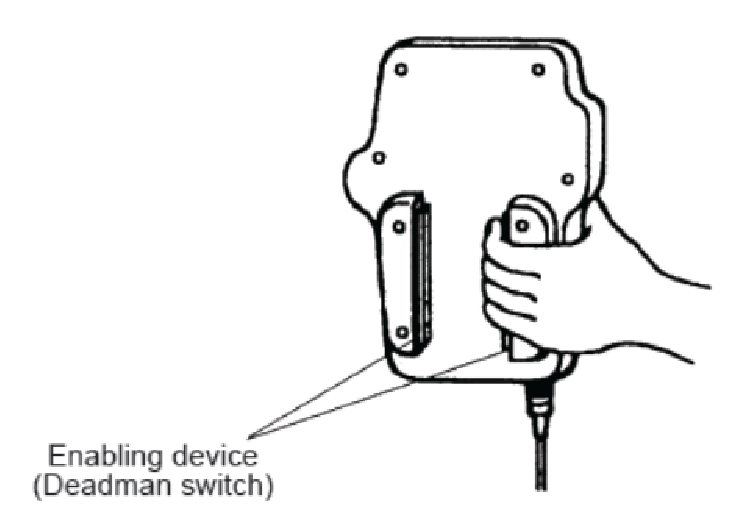
\includegraphics[width=0.5\textwidth]{enabl_device.eps}
	\caption{Varnostno stikalo za vklop motorjev na učni enoti.}
	\label{fig:enabl_device}
\end{figure}

\subsection{Kalibracija orodja} \label{pog:kalibracija_orodja}

Kalibracijo orodja izvedete v meniju \verb|FRAMES|, do katerega pridete preko tipke MENU, nato izberete meni \verb|6 SETUP| in podmeni \verb|3 FRAMES|. Meni potrdite s tipko ENTER. Odpre se okno \verb|FRAMES|. V oknu Frames izberete gumb \verb|OTHER|, ter nato \verb|1 Tool Frame|. Odpre se okno s seznamom orodij. Izberete orodje 9. Odpre se okno za kalibracijo orodja. Pod Comment mora biti izpisano ime \verb|Bela_spica|. Na dnu okna je menijska vrstica. S funkcijsko tipko najprej izberete gumb \verb|METHOD|. Na zaslonu se odpre seznam načinov kalibracije (slika \ref{fig:calib_seznam}):

\begin{itemize}
	\item Three Point
	\item Six Point (XZ)
	\item Six Point (XY)
	\item Two Point + Z
	\item Four Point
	\item Direct Entry
\end{itemize}

\begin{figure}[!hbt]
	\centering
	\includegraphics[width=0.5\textwidth]{IMG_20210827_115248.eps}
	\caption{Okno za izbiro načinov kalibracije in rezultati kalibracije s 4 točkami za orodje {\em Bela\_spica}.}
	\label{fig:calib_seznam}
\end{figure}

\subsubsection{Kalibracija Three Point in Four Point}

Pri tej kalibraciji vrh orodja v 3 oziroma 4 različnih orientacijah premaknemo do kalibracijske špice (glej sliko \ref{fig:tool_3}). Krmilnik nato izračuna točko vrha orodja. Pri tem načinu kalibracije se določi le točka vrha orodja in ne tudi orientacija. Predlagamo izbiro kalibracije s 4 točkami, saj bo tako kalibracija bolj točna, ker bo imel krmilnik na voljo za izračun več podatkov (točk).

\begin{figure}[!hbt]
	\centering
	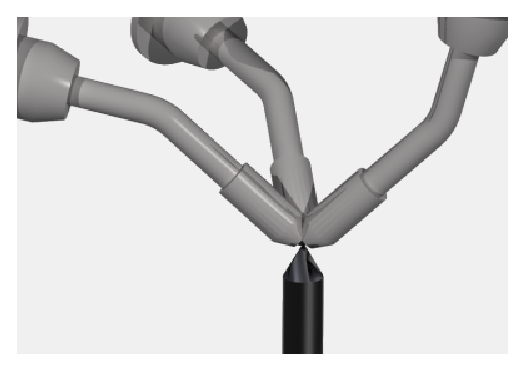
\includegraphics[width=0.5\textwidth]{tool_calibration.eps}
	\caption{Primer kalibracije s tremi točkami. Orodje postavimo v tri različne orientacije, pozicija vrha orodja relativno na kalibracijsko špico pa je ista.}
	\label{fig:tool_3}
\end{figure}

Na zaslonu so izpisane točke za kalibracijo kot Approach point 1 do 4. Pri vsaki točki je zapisano UNINIT (un-initialized). S smernimi tipkami se pomaknemo na izbrano točko. Nato robota premaknemo tako, da se vrh orodja premakne do (in ne dotakne!) kalibracijske špice. Za varen pomik do točke uporabite najprej nizko hitrost ($5\%$ do $10\%$), ko ste blizu točke zmanjšajte hitrost na FINE. Ko ste z lego točke zadovoljni, izberete gumb \verb|RECORD|. Pri točki se izpiše \verb|USED|.

\subsubsection{	Kalibracija Six Point (XZ)}
Pri tej kalibraciji poleg vrha orodja določimo še orientacijo orodja. Poleg treh točk za določitev vrh orodja, so na voljo še tri točke s katerimi določimo x in z-os orodja.

\subsubsection{Kalibacija vijačnega nastavka}
 Kalibracijo orodja za nastavek za vijačenje (glej sliko \ref{fig:nastavek}) je določena s kalibracijo kalibracijske špice, saje je vrh kalibracijske špice na dolžini vrha vijačnega nastavka. Slika \ref{fig:orodje} prikazuje pozicijo vrha kalibracijske špice  in nastavka za vijačenje. Na sliki je prikazan koordinatni sistem vrha orodja (prirobnice), glede na katerega se določi kalibracijo orodja. 

\begin{figure}[!hbt]
	\centering
	\includegraphics[width=0.5\textwidth]{nastavek.eps}
	\caption{Nastavek za vijačenje, ki je sicer skrit v ščitniku nastavka.}
	\label{fig:nastavek}
\end{figure}

\begin{figure}[!hbt]
	\centering
%	\psfrag{tool}[r][r][1.2][0]{nastavek}
%	\psfrag{spike}[r][r][1.2][0]{kalibracijska špica}
	\includegraphics[width=1.0\textwidth]{spica_tool.eps}
	\caption{Sliki prikazujeta kalibracijsko špico in vijačni nastavek. Vrh kalibracijske špice je na istem mestu kot vrh vijačnega nastavka.}
	\label{fig:orodje}
\end{figure}

\newpage

\subsection{Določitev uporabniškega koordinatnega sistema} \label{pog:UF}
Kalibracijo orodja izvedete v meniju FRAMES, do katerega pridete preko tipke MENU, nato izberete meni \verb|6 SETUP| in podmeni \verb|3 FRAMES|. Meni potrdite s tipko ENTER. Odpre se okno \verb|FRAMES|. V oknu Frames izberete gumb \verb|OTHER|, ter nato \verb|3 User Frame|. Odpre se okno s seznamom uporabniških koordinatnih sistemov. Z gumbom \verb|SETIND| lahko izberete aktivni uporabniški koordinatni sistem. Izberete uporabniški koordinatni sistem 5.
 
Z izbiro gumba \verb|METHODS| se nam odpre meni z možnostmi za definicijo uporabniškega koordinatnega sistema:

\begin{itemize}
	\item Three Point,
	\item Four Point,
	\item Direct Entry.
\end{itemize}

Za kalibracijo uporabniškega koordinatnega sistema izberite možnost Three Point. S to opcijo določite tri točke:

\begin{itemize}
	\item Orient Origin Point: izhodišče uporabniškega koordinatnega sistema.
	\item X Direction Point: točka na x-osi uporabniškega koordinatnega sistema.
	\item Y Direction Point: točka na y-osi uporabniškega koordinatnega sistema.
\end{itemize}

\begin{figure}[!hbt]
	\centering
	\includegraphics[width=0.5\textwidth]{UF.eps}
	\caption{Definicija uporabniškega koordinatnega sistema na obdelovancu. Na obdelovancu so nameščene tri kalibracijske špice (označene z rumenimi krogi). Vrh orodja je označen z oranžnim krogom. Smer koordinatnih osi je označena z rdečo puščico za x-os, ter z zeleno y-os.}
	\label{fig:UFrame}
\end{figure}

S tem definirate uporabniški koordinatni sistem, ki ga aktivirate kot aktivnega z izbiro tipke PREV in nato z gumbom \verb|SETIND| odprete možnost za vpis indeksa uporabniškega koordinatnega sistema. Nato preverite, če je definicija uporabniškega koordinatnega sitema uspela. Pojdite v prikaz za lego robota in izberite prikaz glede na uporabniški koordinatni sistem. Izberite tudi premik po oseh uporabniškega koordinatnega sistema z izbiro tipke COORD. Nato se pomaknite v smereh po X in Y smereh, da preverite, če se robot premika v smeri, ki se sklada z uporabniškim koordinatnim sistemom. Nato se pomaknite še nad prvo kalibracijsko špico in preverite če je pozicija robota okoli vrednosti $0$ $mm$. Slika \ref{fig:UF_kalib} prikazuje primer neuspešne in uspešne definicije orodja.


\begin{figure}[!htb]
	\centering
	\psfrag{a}[r][r][1.2][0]{(a)}
	\psfrag{b}[r][r][1.2][0]{(b)}
	\includegraphics[width=0.75\textwidth]{UF_kalib.eps}
	\caption{Primer (a) neuspešne in (b) uspešne definicije orodja.}
	\label{fig:UF_kalib}
\end{figure}



\subsection{Pisanje programa}
Napisali boste testni program z različnimi vrstami premikov robota v različne točke. Primer postavitve petih točk je prikazan na sliki \ref{fig:prog2}.

\begin{itemize}
	\item Točka P1: točka naj bo postavljena najvišje in nad delovnim objektom na katerem ste definirali uporabniški koordinatni sistem. V to točke se boste premaknili z ukazom za gibanje po sklepih.
	\item Točka P2: Točka naj bo postavljena pod točko P1. V to točko se boste pomaknili z linearnim gibom, točka naj bo definirana v koordinatnem sistemu robota.
	\item Točke P3, P4 in P5: Točke si postavljene $3-5$ $cm$ nad delovnim objektom v trikotni porazdelitvi in so definirane v uporabniškem koordinatnem sistemu.
\end{itemize}

\begin{figure}[!hbt]
	\centering
	\includegraphics[width=0.8\textwidth]{prog3.eps}
	\caption{Primer razporeditve točk.}
	\label{fig:prog2}
\end{figure}

Slika \ref{fig:prog2} z rdečimi puščicami prikazuje vrstni red premikov robota:

\begin{enumerate}
	\item premik: premik v točko P1 s premikom po sklepih.
	\item premik: premik v točko P2 z linearnim premikom v koordinatnem sistemu robota.
	\item premik: premik v točko P3 z linearnim premikom v uporabniškem koordinatnem sistemu.	
	\item premik: premik v točko P4 z linearnim premikom v uporabniškem koordinatnem sistemu.	
	\item premik: premik v točko P5 z linearnim premikom v uporabniškem koordinatnem sistemu.	
	\item premik: premik v točko P2 z linearnim premikom v koordinatnem sistemu robota.	
	\item premik: premik v točko P1 s premikom po sklepih.	
\end{enumerate}	

Najprej prekličite izbiro uporabniškega koordinatnega sistema, da bo točka shranjena v baznem koordinatnem sistemu robota.

Program začnete pisati tako, da izberete tipko SELECT na ročni učni enoti. Odpre se seznam z ustvarjenimi programi in menijska vrstica na dnu, kjer lahko gumbe izbirate s funkcijskimi tipkami. Z izbiro gumba \verb|CREATE| (tipka F2) ustvarite nov program. 

Sedaj ustvarite testni program. Edina vrstica, ki se vam prikaže je vrstica \verb|[End]|, ki nakazuje konec programa (glej sliko \ref{fig:program}(a)). Ko se postavite na to vrstico in izberete nov ukaz, ga bo postavilo pred izbrano vrstico. Robot premaknete v želeno prvo točko, izberete ikono POINT, ki vam ponudi meni z možnostim za različne gibe (glej sliko \ref{fig:program}(b)). Izberete \verb|J P[] 100% FINE| možnost. Za naslednjo točko pomaknite robota po z-osi globalnga koordinatnega sistema navzdol in shranite novo točko kot točko 2. Izberete možnost \verb|L P[] 100mm/sec FINE|.

Preverite, če je točka 2 res definirana v baznem koordinatnem sistemu robota. S smernimi tipkami na učni enoti se premaknite na indeks točke (glej sliko \ref{fig:program}(c)). Izberete ikono \verb|POSITION|. Odpre se okno s podatki o točki (glej sliko \ref{fig:program}(d)). Slika \ref{fig:program}(e) prikazuje primer za točko 5. Za definiranje točk v uporabniškem koordinatnem sistemu je potrebno izbrati ustrezen uporabniški koordinatni sistem. Izberite uporabniški koordinatni sistem, ki ste ga definirali. Tipka MENU, \verb|6  SETUP|, \verb|3 Frames|. Odpre se novo okno, izberete ikono \verb|OTHER|, nato \verb|3  User Frame|. Odpre se okno z uporabniškimi koordinatnimi sistemi \verb|SETUP Frames|. Z izbiro ikone \verb|SETIND| izberete indeks vašega uporabniškega koordinatnega sistema. Nato nadaljujete s pisanjem programa. Izberete tipko SELECT in vaš program. Premaknite se na vrstico \verb|[End]| in nadaljujete z dodajanjem točk. 

\begin{figure}[!hbt]
	\centering
	\psfrag{a}[c][c][1][0]{(a)}
	\psfrag{b}[c][c][1][0]{(b)}		
	\psfrag{c}[c][c][1][0]{(c)}
	\psfrag{d}[c][c][1][0]{(d)}
	\psfrag{e}[c][c][1][0]{(e)}	
	\psfrag{f}[c][c][1][0]{(f)}			
	\includegraphics[width=1.0\textwidth]{program.eps}
	\caption{(a) Začetno okno za pisanje programa. (b) Izbira vrste giba. (c) Izbira indeksa točke za preverjanje v katerem koordinatnem sistemu je točka definirana. (d) Podatki za izbrano točko, ki je definirana v baznem koordinatnem sistemu robota. (e) Podatki za izbrano točko, ki je definirana v uporabniškem koordinatnem sistemu. (f) Program za premikanje po poti predstavljeni na sliki \ref{fig:prog2}.}
	\label{fig:program}
\end{figure}

Na koncu dodajte novo točko, ki jo shranilo pod indeks 6. Če se premaknete na indeks in izberete tipko 2, boste zamenjali indeks točke. Končan program je prikazan na sliki \ref{fig:program}(f). Program testirate tako, da se pomaknete na prvo vrstico ter držite tipko SHIFT in FWD. Robot se bo premikal po izbranih vrsticah.

\subsection{Program za vijačenje vijaka}

\subsubsection{Korak 1} Kalibracija kalibracijske špice (glej poglavje \ref{pog:kalibracija_orodja}).
\subsubsection{Korak 2} Določitev uporabniške koordinatnega sistema (glej poglavje \ref{pog:UF}).
\subsubsection{Korak 3} Pisanje programa, ki je opisan spodaj. 

\vspace{0.35cm}
\begin{mdframed}[backgroundcolor=red!20, shadow=true,roundcorner=8pt]
	
Za pripravo programa naj bo zaščita za vijačnik izklopljena, izklopljena mora biti tudi varnost. \newline ODSTRANI ZAŠČITO IN IZKLOPI VARNOST LAHKO LE ASISTENT!
	
\end{mdframed}

Začnite pisati nov program.

\begin{figure}[!hbt]
	\centering
	\psfrag{a}[c][c][1][0]{(a)}
	\psfrag{b}[c][c][1][0]{(b)}		
	\psfrag{c}[c][c][1][0]{(c)}
	\psfrag{d}[c][c][1][0]{(d)}
	\psfrag{e}[c][c][1][0]{(e)}	
	\psfrag{f}[c][c][1][0]{(f)}			
	\psfrag{g}[c][c][1][0]{(g)}
	\psfrag{h}[c][c][1][0]{(h)}
	\includegraphics[width=1.0\textwidth]{kolaz2-1.eps}
	\caption{Izvajanje programa za vijačenje}
	\label{fig:kolaz2-1}
\end{figure}

\begin{figure}[!hbt]
	\centering
	\psfrag{i}[c][c][1][0]{(i)}
	\psfrag{j}[c][c][1][0]{(j)}		
	\psfrag{k}[c][c][1][0]{(k)}
	\psfrag{l}[c][c][1][0]{(l)}
	\psfrag{m}[c][c][1][0]{(m)}	
	\includegraphics[width=1.0\textwidth]{kolaz2-2.eps}
	\caption{Izvajanje programa za vijačenje}
	\label{fig:kolaz2-2}
\end{figure}

Na začetku je potrebno vklopiti digitalne izhode, ki so povezani na PLK, ki skrbi za varnost, ter digitalni izhod, ki je povezan z krmlnikom za vijačnik. V ukazni vrstici na dnu zaslona izberete \verb|[INST]| (tipka F1). Odpre se meni za izbiro različni ukazov, ki so razdeljeni v skupine (glej sliko \ref{fig:DO}(a)). Izberete \verb|I/O|, nato \verb|DO[ ]=...| (glej sliko \ref{fig:DO}(b)). Premaknite se na prazno polje med oglatimi oklepaji in vpišite ustrezen digitalni izhod. Nato se premaknete na mesto za izbiro \verb*|On/Off| možnosti \textbf{(glej sliko \ref{fig:DO}c))}. 

\begin{figure}[!hbt]
	\centering
	\psfrag{a}[c][c][1][0]{(a)}
	\psfrag{b}[c][c][1][0]{(b)}		
	\psfrag{c}[c][c][1][0]{(c)}
	\includegraphics[width=1.0\textwidth]{DO.eps}
	\caption{Izbira digitalnih izhodov.}
	\label{fig:DO}
\end{figure}

Dodajte kodo za izbiro treh digitalnih izhodov, kot je prikazano v nadaljevanju.

\vspace{0.35cm}
\begin{mdframed}[backgroundcolor=orange!20, shadow=true,roundcorner=8pt]

\begin{verbatim}
	1:  DO[120:OFF:SAFE_START]=OFF ;
	2:  DO[127:OFF:PR3]=OFF ;
	3:  DO[116:ON :XHOLD]=ON ;
\end{verbatim}
	
\end{mdframed}

Dodali boste prvo točko, ki bo definirana v baznem koordinatnem sistemu (\verb*|UFRAME_NUM=0|) in glede na prirobnico robota (\verb*|UTOOL_NUM=1|).
\begin{itemize}
	\item Izbira baznega koordintnega sistema:  tipka MENU, \verb|6  SETUP|, \verb|3 Frames|. Odpre se novo okno, izberete ikono \verb|OTHER|, nato \verb|3  User Frame|. Odpre se okno z uporabniškimi koordinatnimi sistemi \verb|SETUP Frames|. Bazni koordinatni sistem izberete tako, da se s tipko NEXT se premaknete na naslednjo stran spodnje menijske vrstice in izberet ikono \verb*|CLRIND|.
	\item Izbira koordinatnega sistema orodja prirobnice: tipka MENU , \verb|6  SETUP|, \verb|3 Frames|. Odpre se novo okno, izberete ikono \verb|OTHER|, nato \verb|1  Tool Frame|.  Odpre se okno s seznamom orodij. Z izbiro ikone \verb*|SETIND| izberete orodje 1. 
\end{itemize}

Sedaj se vrnete v svoj program s tipko SELECT in izberet vaš program. V programu boste dodali vrstici za izbiro ustreznih koordinatnih sistemov. V ukazni vrstici na dnu zaslona izberete \verb|[INST]| (tipka F1), nato \verb*|4 Offset/Frames|. Izberete ustrezne ukaze in vrednosti kot je prikazano spodaj.

\vspace{0.35cm}
\begin{mdframed}[backgroundcolor=orange!20, shadow=true,roundcorner=8pt]
	
	\begin{verbatim}
	4:  UFRAME_NUM=0 ;
	5:  UTOOL_NUM=1 ;
	\end{verbatim}
	
\end{mdframed}

Robota postavite v točko nad obdelovancem kot je prikazano na sliki \ref{fig:kolaz2-1}(a). Za premik v to točko izberite premik po sklepih, spremenite še hitrost. 

\vspace{0.35cm}
\begin{mdframed}[backgroundcolor=orange!20, shadow=true,roundcorner=8pt]
	
	\begin{verbatim}
	6:J P[1] 5% FINE    ;
	\end{verbatim}
	
\end{mdframed}

Sedaj boste klicali program za pobiranje orodja nastavka za vijačenje.  V ukazni vrstici na dnu zaslona izberete \verb|[INST]| (tipka F1), nato \verb*|6 CALL|. V novem oknu izberete ukaz \verb*|CALL program|. Odpre se okno s seznamom programov, izberet program \verb*|PICK_TOOL_1|. Ta program bo izvedel sekvenco pobiranja nastavka, ki je prikazan na slikah \ref{fig:kolaz2-1}(b) do (d). Naslednji ukaz je premik v točko 1. Dodate nov ukaz za premik, ki vam tudi shrani novo točko. Premaknete se na indeks nove točke in ji spremenite indeks na 1.

\vspace{0.35cm}
\begin{mdframed}[backgroundcolor=orange!20, shadow=true,roundcorner=8pt]
	
	\begin{verbatim}
	7:  CALL PICK_TOOL_1    ;
	8:J P[1] 5% FINE    ;
	\end{verbatim}
	
\end{mdframed}

V nadaljevanju boste delali v koordinatnem sistemu obdelovanca (\verb*|UFRAME_NUM=5|) in z orodjem kalibracijske špice (\verb*|UTOOL_NUM=9|). 

\begin{itemize}
	\item Izbira koordintnega sistema obdelovanca:  tipka MENU, \verb|6  SETUP|, \verb|3 Frames|. Odpre se novo okno, izberete ikono \verb|OTHER|, nato \verb|3  User Frame|. Odpre se okno z uporabniškimi koordinatnimi sistemi \verb|SETUP Frames|. Koordinatni sistem obdelovanca izberete tako, da v spodnje menijske vrstice izberet ikono \verb*|SETIND| in izberete indeks 5.
	\item Izbira koordinatnega sistema orodja prirobnice: tipka MENU , \verb|6  SETUP|, \verb|3 Frames|. Odpre se novo okno, izberete ikono \verb|OTHER|, nato \verb|1  Tool Frame|.  Odpre se okno s seznamom orodij. Z izbiro ikone \verb*|SETIND| izberete orodje 9. 
\end{itemize}

Sedaj se vrnete v svoj program s tipko SELECT in izberet vaš program. V programu boste dodali vrstici za izbiro ustreznih koordinatnih sistemov. V ukazni vrstici na dnu zaslona izberete \verb|[INST]| (tipka F1), nato \verb*|4 Offset/Frames|. Izberete ustrezne ukaze in vrednosti kot je prikazano spodaj.

\vspace{0.35cm}
\begin{mdframed}[backgroundcolor=orange!20, shadow=true,roundcorner=8pt]
	
	\begin{verbatim}
	9:  UTOOL_NUM=9 ;
	10:  UFRAME_NUM=5 ;
	\end{verbatim}
	
\end{mdframed}

Sedaj postavite digitalni izhod na indeksu 127 na stanje ON.

\vspace{0.35cm}
\begin{mdframed}[backgroundcolor=orange!20, shadow=true,roundcorner=8pt]
	
	\begin{verbatim}
	11:  DO[127:OFF:PR3]=ON ;
	\end{verbatim}
	
\end{mdframed}

Če na vijačniku ni kalibracijske špice, jo namestimo nazaj na vijačnik. V luknjo z navojem zavijte vijak, nato pa se s kalibracijsko špico pomaknete do zavitega vijaka (glej sliko \ref{fig:tocka_vijak}) in shranite točko z ukazom za linearni pomik. 

\begin{figure}[!hbt]
	\centering
	\includegraphics[width=0.5\textwidth]{tocka_vijak.eps}
	\caption{Določanje točke za privijačenje vijaka.}
	\label{fig:tocka_vijak}
\end{figure}

Ker se želimo najprej pomakniti nad vijak (glej sliko \ref{fig:kolaz2-1}(f)), bomo točki dodali odmik v smeri z osi. Odmik je shranjen v točkovnem registru \verb*|PR[24]|. Pomaknite se na konec vrstice (glej sliko \ref{fig:point_offset}(a)) in izberite ikono \verb*|[CHOICE]|. Odpre se meni prikazan na sliki \ref{fig:point_offset}(b), izberete \verb*|7 Offset,PR[ ]|. Vpišite številko odmika.

\begin{figure}[!hbt]
	\centering
	\psfrag{a}[c][c][1][0]{(a)}
	\psfrag{b}[c][c][1][0]{(b)}		
	\psfrag{c}[c][c][1][0]{(c)}	
	\includegraphics[width=0.7\textwidth]{point_offset.eps}
	\caption{Določanje točke za privijačenje vijaka.}
	\label{fig:point_offset}
\end{figure}

Dodajte še en linearen pomik do odmika do odmika na indeksu \verb*|PR[38]|. To je domik, ki je nekaj mm nad točko, ko se zaščita dotakne aluminijastega obdelovanca. Zmanjšajte hitrost na $10$ $mm/sec$. Ukaza sta prikazana spodaj.

\vspace{0.35cm}
\begin{mdframed}[backgroundcolor=orange!20, shadow=true,roundcorner=8pt]
	
	\begin{verbatim}
	12:L P[2] 100mm/sec FINE Offset,PR[24:VAJA_NEBRISI1   ]    ;
	13:L P[2] 10mm/sec FINE Offset,PR[38:VAJA_NEBRISI3  ]    ;
	\end{verbatim}
	
\end{mdframed}

Nato je potrebno izključiti detekcijo trka zaščite. Digitalni izhod na indeksu 116 je potrebno postaviti na \verb*|ON|.

\vspace{0.35cm}
\begin{mdframed}[backgroundcolor=orange!20, shadow=true,roundcorner=8pt]
	
	\begin{verbatim}
	14:  DO[116:ON :XHOLD]=ON ;
	\end{verbatim}
	
\end{mdframed}

Dodajte še en linearen pomik do odmika \verb*|PR[26]|, ki je tik nad vijakom (glej sliko \ref{fig:kolaz2-1}(g)).

\vspace{0.35cm}
\begin{mdframed}[backgroundcolor=orange!20, shadow=true,roundcorner=8pt]
	
	\begin{verbatim}
	15:L P[2] 10mm/sec FINE Offset,PR[26:VAJA_NEBRISI2]    ;
	\end{verbatim}
	
\end{mdframed}

Nato lahko izklopite varnost (digitalni izhod 120 na \verb*|ON|) in zaženete vijačnik (digitalni izhod 81 na \verb*|ON|).

\vspace{0.35cm}
\begin{mdframed}[backgroundcolor=orange!20, shadow=true,roundcorner=8pt]
	
	\begin{verbatim}
	16:  DO[120:OFF:SAFE_START]=ON ;
	17:  DO[81:OFF]=ON ;
	\end{verbatim}
	
\end{mdframed}

Sedaj lahko dodate ukaz za pomik v končno točko za zavijačenje vijaka. Hitrost zmanjšajte na $3$ $mm/sec$.

\vspace{0.35cm}
\begin{mdframed}[backgroundcolor=orange!20, shadow=true,roundcorner=8pt]
	
	\begin{verbatim}
	18:L P[2] 3mm/sec FINE    ;
	\end{verbatim}
	
\end{mdframed}

Dodajte še ukaz, da po koncu vijačenja robot obstane v končni točki za 1 sekundo. Do ukaza pridemo z \verb|[INST]|, nato \verb*|3 WAIT|, ter nazadnje \verb*|1 WAIT ... (sec)|. Pomaknemo se na vrednost \verb*|0.00 (sec)| in vtipkamo vrednost 1.

\vspace{0.35cm}
\begin{mdframed}[backgroundcolor=orange!20, shadow=true,roundcorner=8pt]
	
	\begin{verbatim}
	  19:  WAIT   1.00(sec) ;
	\end{verbatim}
	
\end{mdframed} 

Krmilnik vijačnika bo zaznal, da je vijak zavit, saj bo narasel potreben navor za zavijanje. Ko bo navor presegel določeno vrednost, ki je vnaprej določena na krmilniku vijačnika, se bo vijačenje ustavilo. Kljub temu je potrebno izklopiti program za vijačenje z vpisom vrednosti \verb*|OFF| na digitalni izhod 127. Nazaj lahko vključimo tudi varnost z vpisom \verb*|OFF| na digitalni izhod 120.

\vspace{0.35cm}
\begin{mdframed}[backgroundcolor=orange!20, shadow=true,roundcorner=8pt]
	
	\begin{verbatim}
	20:  DO[127:OFF:PR3]=OFF ;
	21:  DO[120:OFF:SAFE_START]=OFF ;
	\end{verbatim}
	
\end{mdframed} 

Sedaj lahko vijačnik dvignemo z linearnim pomikom na višino odmika \verb*|PR[24]| (glej sliko \ref{fig:kolaz2-2}(i)) in zklopimo digitalna izhoda 81 in 166.

\vspace{0.35cm}
\begin{mdframed}[backgroundcolor=orange!20, shadow=true,roundcorner=8pt]
	
	\begin{verbatim}
	22:L P[2] 100mm/sec FINE Offset,PR[24:VAJA_NEBRISI1   ]    ;
	23:  DO[81:OFF]=OFF ;
	24:  //DO[116:ON :XHOLD]=OFF ;
	\end{verbatim}
	
\end{mdframed} 

Sedaj lahko robota pomaknemo nad obdelovanca v točko 1 (glej sliko \ref{fig:kolaz2-2}(j)). Še prej pa je potrebno spremeniti uporabniški koordinatni sistem v bazni koordinatni sistem robota ter spremeniti koordinatni sistem orodja v koorsinatni sistem prirobnice.

\vspace{0.35cm}
\begin{mdframed}[backgroundcolor=orange!20, shadow=true,roundcorner=8pt]
	
	\begin{verbatim}
	25:  UTOOL_NUM=1 ;
	26:  UFRAME_NUM=0 ;
	27:J P[1] 5% FINE 
	\end{verbatim}
	
\end{mdframed} 

Sedaj lahko odložimo vijačni nastavek s klicem programa \verb*|PLACE_TOOL_1| (glej sliki \ref{fig:kolaz2-2}(k) in (l)).

\vspace{0.35cm}
\begin{mdframed}[backgroundcolor=orange!20, shadow=true,roundcorner=8pt]
	
	\begin{verbatim}
	28:  CALL PLACE_TOOL_1    ;
	\end{verbatim}
	
\end{mdframed} 

Za konec se spet pomaknemo v točko 1 (glej sliko \ref{fig:kolaz2-2}(m)).

\vspace{0.35cm}
\begin{mdframed}[backgroundcolor=orange!20, shadow=true,roundcorner=8pt]
	
	\begin{verbatim}
	29:J P[1] 5% FINE    ;
	\end{verbatim}
	
\end{mdframed} 

S tem je program za zavijanje enega vijaka končan. 

\subsubsection{Korak 4} Zagon programa

\vspace{0.35cm}
\begin{mdframed}[backgroundcolor=red!20, shadow=true,roundcorner=8pt]
	
POKLIČITE ASISTENTA, DA BO OB ZAGONU PROGRAMA ZRAVEN.
	
\end{mdframed}

Sedaj lahko program zaženete. Vijak nastavite v luknjo, tako da je nekoliko zavit v navoj, vendar le toliko, da stoji stabilno pokonci. Hitrost izvajanja programa postavite na $100$ $\%$. Pomaknite se na prvo vrstico programa. Vklopite varnostno stikalo na zadnji strani učne enote, pritisnete tipko RESET, da se vklopijo motorji. Nato držite tipko SHIFT in FWD. Če se na zaslonu pojavi vprašanje ali želite začeti iz izbrane vrstice programa s tipko ENTER potrdite, nato pa še enkrat kliknete na tipko FWD. Program se bo izvedel.

\subsubsection{Korak 5} Po zgornjem vzoru dodajte ustrezne ukaza za zavijanje še enega vijaka.